%------------------------------------ Inicio ---------------------------------------
\documentclass[11pt, a4paper]{article}

% -------------- Nombre del documento --------------
\newcommand{\nombre}{Trabajo Final Integrador}
%---------------------------------------------------------

%-------------------- Include Paquetes iniciales---------------------
\usepackage{mathtools}
\usepackage{graphicx}
\usepackage{float} 
\usepackage{geometry}
\geometry{top=30mm,bottom=30mm,left=33mm,right=33mm,headsep=15mm}
\usepackage{relsize} % agranda a un mas las letras
\usepackage[spanish,es-nodecimaldot]{babel}
\usepackage[utf8]{inputenc}
\usepackage{lastpage} % nos dice el numero total de paginas
\usepackage{fancyhdr} % modifica encabezado y pie de pagina
\usepackage{siunitx} % para \si y \SI
\usepackage{pdfpages} % Para adjuntar datasheets
%\usepackage[hidelinks]{hyperref} % moved later to avoid LaTeX hooks conflicts
\usepackage{booktabs}
% --- NUEVA TIPOGRAFÍA RECOMENDADA: Palatino ---
%\usepackage{mathpazo} 
%\usepackage{mathptmx}
\usepackage{lmodern}
% Si prefieres Times, comenta la línea de arriba y usa: \usepackage{mathptmx}
\usepackage{multirow}
\usepackage{graphicx}
\usepackage{makecell}
\usepackage{enumitem}
\usepackage{svg}
% ----------------------------------------------

% Estilos de página
\pagestyle{fancy} 
\renewcommand{\headrulewidth}{0.1pt} 
\renewcommand{\footrulewidth}{0pt} 

% Para tablas formato:
\usepackage[table]{xcolor} 
\renewcommand{\arraystretch}{1.4} % espaciado vertical

\setlength{\headheight}{25.61053pt}
\cfoot{}
\pagestyle{fancy}
\fancyhf{}
\rfoot{\thepage}
\lhead{
\includegraphics[scale=0.11]{Imagenes/logoPrincipal.jpg}}
\rhead{\nombre}

%Python
\usepackage{listings}
% \usepackage{xcolor}

% Definición de colores para el código
\definecolor{codegreen}{rgb}{0,0.6,0}
\definecolor{codegray}{rgb}{0.5,0.5,0.5}
\definecolor{codepurple}{rgb}{0.58,0,0.82}
\definecolor{backcolour}{rgb}{0.95,0.95,0.92}

% Estilo para el código Python
\lstdefinestyle{mystyle}{
    backgroundcolor=\color{backcolour},   
    commentstyle=\color{codegreen},
    keywordstyle=\color{blue},
    numberstyle=\tiny\color{codegray},
    stringstyle=\color{codepurple},
    basicstyle=\ttfamily\footnotesize, % Fuente tipo máquina de escribir
    breakatwhitespace=false,         
    breaklines=true,                 
    captionpos=b,                    
    keepspaces=true,                 
    numbers=left,                    
    numbersep=5pt,                  
    showspaces=false,                
    showstringspaces=false,
    showtabs=false,                  
    tabsize=2,
    language=Python
}

\lstset{style=mystyle}

% Bibliografia
\usepackage[style=apa]{biblatex}
\usepackage{csquotes}
\addbibresource{bibliografia.bib}

%-----------------------------------------------------------------------
% Ensure proper caption handling to avoid LaTeX hooks error with hyperref
\usepackage{caption}

% Load hyperref last to avoid LaTeX hooks conflicts
\usepackage[hidelinks]{hyperref} % Para que funcionen los links \url{} en la bibliografía

\begin{document}

%--------------------  Portada ---------------------
\begin{center}
	\vspace*{10mm}
	\textscale{2}{ \textbf{\nombre}} \\
	\vspace{6mm}
	\textscale{1.6}{ Electrónica Industrial }\\
	\vspace{4mm}
	\textscale{1.3}{2026}\\
    ---------------------------

    \textbf{\begin{figure}[H]
		\centering
		
\includegraphics[width=0.4\linewidth]{Imagenes/unc_logo_solo.png}
	\end{figure}}
    
    \vspace*{8mm}
    {\Large \textbf{Autores}} \\
    \vspace{4mm}

    \renewcommand{\arraystretch}{2}
    \begin{tabular}{lll}
        Cabero, Mauro Ezequiel & 43761887 \\
        Testa, Lisandro  & 43477019 \\
        Zúñiga, Guillermo Rubén Darío  & 44229491 \\
    \end{tabular}

    \vspace{15mm}

    {\Large \textbf{Docentes}} \\
    \vspace{8mm}

    \begin{minipage}{0.5\linewidth}
        \centering
        Ing. Esp. Adrián Agüero
    \end{minipage}

    \vfill 
    \thispagestyle{empty}
\end{center} % <--- AQUÍ SE CIERRA EL ÚNICO ENTORNO CENTER DE LA PORTADA
\clearpage

\tableofcontents
\thispagestyle{empty}
\clearpage

% ------------------------------------- Desarrollo ---------------------------------
\pagenumbering{arabic}

\section{Introducción}

El crecimiento sostenido de las energías renovables y los sistemas de almacenamiento de energía ha impulsado la necesidad de desarrollar convertidores electrónicos de potencia cada vez más eficientes y versátiles. En este contexto, los convertidores DC-DC bidireccionales desempeñan un papel fundamental al permitir la transferencia controlada de energía entre diferentes fuentes y sistemas de almacenamiento, adaptándose a una amplia variedad de aplicaciones industriales, residenciales y de movilidad eléctrica.

Entre las distintas topologías disponibles, el convertidor \textit{Dual Active Bridge} (DAB) ha adquirido una relevancia creciente debido a sus características de aislamiento galvánico mediante transformador de alta frecuencia, capacidad de transferencia bidireccional de potencia, amplio rango de adaptación de tensión y elevada densidad de potencia. Estas ventajas lo convierten en una solución ampliamente utilizada en sistemas de almacenamiento energético, cargadores bidireccionales para vehículos eléctricos y aplicaciones vinculadas a redes eléctricas inteligentes.

La topología DAB está compuesta por dos puentes activos completos conectados mediante un transformador de alta frecuencia y una inductancia serie, permitiendo controlar tanto la magnitud como el sentido del flujo de potencia mediante técnicas de modulación por desfase. Gracias a esta característica, es posible operar el convertidor tanto en modo elevador como reductor de tensión, manteniendo el aislamiento eléctrico entre sus puertos de entrada y salida.

En el presente trabajo se aborda el estudio, diseño y simulación de un convertidor DC-DC bidireccional basado en la topología DAB para una tensión de entrada de \SI{48}{V}, una tensión de salida de \SI{400}{V} y un rango de corriente de hasta \SI{40}{A}. Para ello se analizan los principios de funcionamiento de la topología, se seleccionan los componentes principales del sistema, se desarrolla el circuito de control y disparo de los dispositivos de potencia, y finalmente se verifican los resultados obtenidos mediante simulación comparándolos con los valores teóricos calculados.

\section{Objetivos}

\subsection{Objetivo General}

Diseñar y simular un convertidor DC-DC bidireccional basado en la topología \textit{Dual Active Bridge} (DAB), destinado a la transferencia de energía entre una fuente de corriente continua de \SI{48}{V} y una carga de \SI{400}{V} con un rango de corriente de hasta \SI{40}{A}. El desarrollo contempla el análisis teórico de la topología, el dimensionamiento de los componentes principales del circuito de potencia, el diseño de las etapas de control y disparo de los dispositivos semiconductores, y la validación de su funcionamiento mediante simulaciones eléctricas.

\subsection{Objetivos Específicos}

\begin{enumerate}
\item Investigar el principio de funcionamiento de los convertidores DC-DC bidireccionales y analizar las características de la topología Dual Active Bridge.

\item Estudiar las estrategias de control utilizadas en convertidores DAB, con énfasis en la modulación por desplazamiento de fase (\textit{Single Phase Shift}).

\item Determinar las especificaciones eléctricas del sistema a partir de los requerimientos de tensión, corriente y potencia establecidos.

\item Dimensionar los elementos principales del circuito de potencia, incluyendo transformador de alta frecuencia, inductancias, capacitores y dispositivos semiconductores.

\item Seleccionar los dispositivos de potencia y los circuitos auxiliares necesarios para garantizar una operación segura y eficiente del convertidor.

\item Desarrollar el circuito de control encargado de generar las señales PWM necesarias para la operación del convertidor.

\item Implementar el modelo completo del convertidor en un entorno de simulación y verificar su funcionamiento.

\item Analizar las formas de onda obtenidas y comparar los resultados de simulación con los valores teóricos calculados.
\end{enumerate}

\section{Marco Teórico}

El convertidor de doble puente activo (DAB) tiene la topología de la figura \ref{fig:circuito}. Está compuesto por una etapa inversora y otra rectificadora, con ambas etapas consistiendo de un puente H que puede ser comúnmente de mosfets o IGBT, y con un transformador de alta frecuencia enmedio. Este circuito es utilizado para transferir potencia de un lado de baja tensión a otro de alta tensión y viceversa, mientras provee un aislamiento galvánico entre ellos.



\begin{figure}[H]
    \centering
    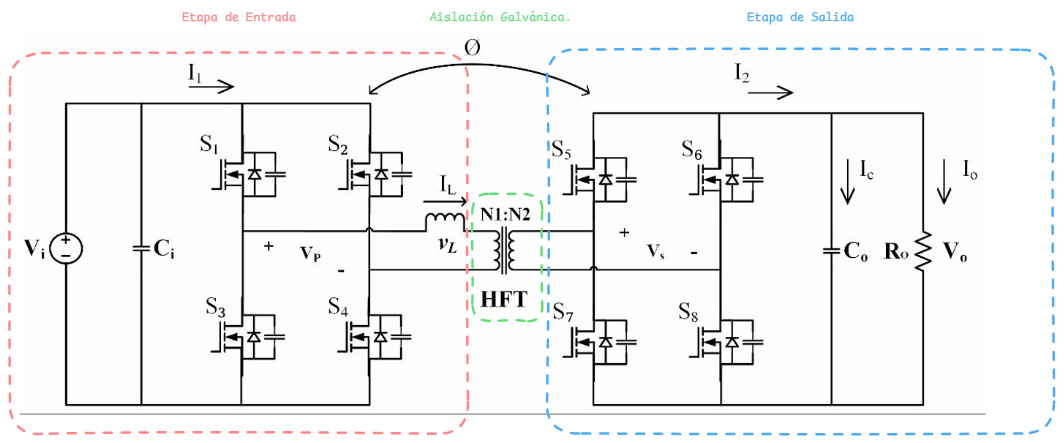
\includegraphics[width=0.8\linewidth]{Imagenes/circuito.png}
    \caption{cap (\cite{kulkarni}).}
    \label{fig:circuito}
\end{figure}

\section{Selección de Componentes}


\begin{figure}[H]
    \centering
    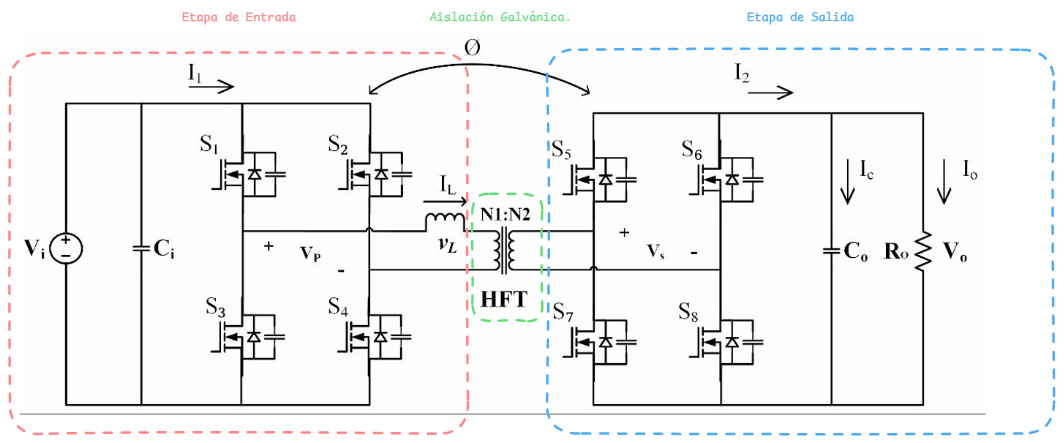
\includegraphics[width=0.8\linewidth]{Imagenes/circuito.png}
    \caption{cap.}
    \label{fig:circuito}
\end{figure}

\section{Desarrollo del Driver}


\section{Resultados en Simulación}

\begin{figure}
    \centering
    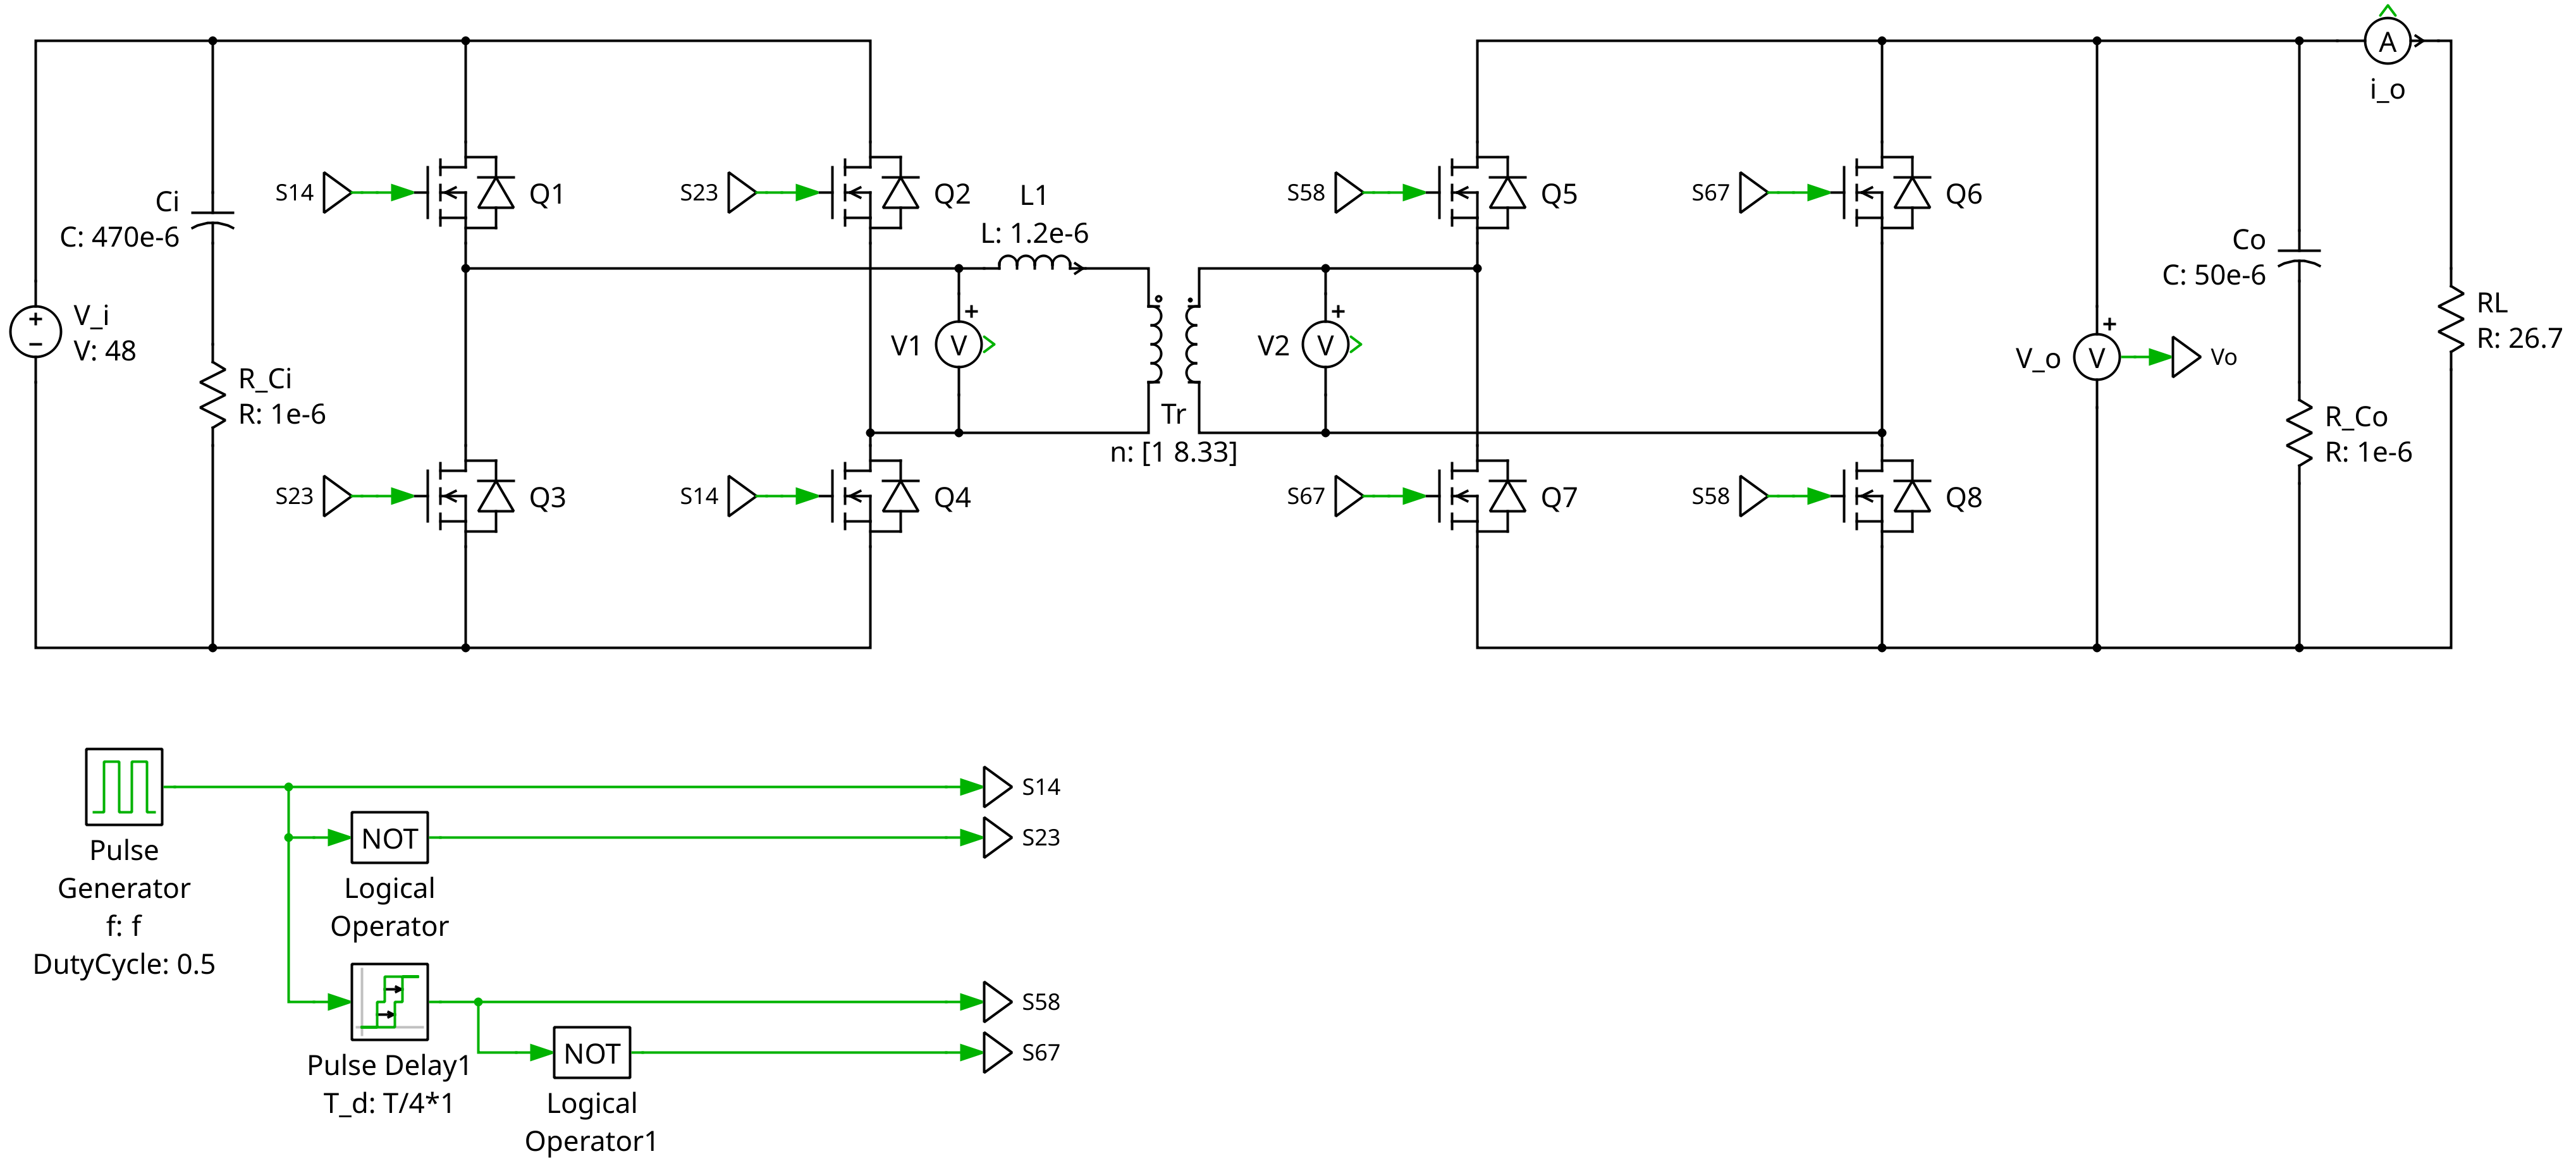
\includegraphics[width=1\linewidth]{Imagenes/circuito_sim.png}
    \caption{cap}
    \label{fig:circuito_sim}
\end{figure}

\section{Conclusión}



%\newpage
%\begin{thebibliography}{9}

%\bibitem{manual_g110_es}
%Siemens AG. ``Convertidor de frecuencia compacto SINAMICS G110 - Instrucciones de servicio (Resumen).'' Edición 04/2004. \\
%\url{https://cache.industry.siemens.com/dl/files/608/18947608/att_66221/v1/G110_COM_18947608__sp_0404.pdf}

%\end{thebibliography}
\nocite{*}
\printbibliography[title={Bibliografía}]

\end{document}
% ------------------------------------- Desarrollo ---------------------------------

% COMANDOS UTILES

\begin{table}[H]
\centering
\caption{Parámetros fundamentales del SINAMICS G110 para puesta en servicio rápida.}
\resizebox{0.85\textwidth}{!}{%
\begin{tabular}{@{} lcc @{}}
\toprule
\textbf{Parámetro} & \textbf{Nombre / Descripción} & \textbf{Nivel de acceso} \\
\midrule
P0100 & Selección de región geográfica (Frecuencia de red: 50 Hz o 60 Hz) & 1 \\
P0304 & Tensión nominal del motor [V] de la placa de características & 1 \\
P0305 & Corriente nominal del motor [A] de la placa de características & 1 \\
P0307 & Potencia nominal del motor [kW / hp] de la placa de características & 1 \\
P0308 & Factor de potencia ($\cos\varphi$) nominal del motor de placa & 3 \\
P0309 & Rendimiento nominal del motor [\%] de la placa de características & 3 \\
P0310 & Frecuencia nominal del motor [Hz] de la placa de características & 1 \\
P0311 & Velocidad nominal del motor [rpm] de la placa de características & 1 \\
P0335 & Tipo de refrigeración del motor (Autoventilado o Ventilación forzada) & 3 \\
P0640 & Factor de sobrecarga del motor [\%] respecto a la nominal P0305 & 3 \\
P0700 & Selección de fuente de órdenes (0: Fábrica, 1: BOP, 2: Terminales, 5: USS) & 1 \\
P1000 & Selección de consigna de frecuencia (1: MOP, 2: Analógica, 3: Fija, 5: USS) & 1 \\
P1080 & Frecuencia mínima del motor [Hz] a la cual funcionará & 1 \\
P1082 & Frecuencia máxima del motor [Hz] límite de operación & 1 \\
P1120 & Tiempo de aceleración [s] desde parado hasta frecuencia máxima & 1 \\
P1121 & Tiempo de deceleración [s] desde frecuencia máxima hasta parado & 1 \\
P1135 & Tiempo de deceleración ante parada de emergencia OFF3 [s] & 3 \\
P1300 & Modo de control (0: V/f lineal, 2: V/f cuadrático, 3: V/f programable) & 2 \\
P3900 & Fin de puesta en servicio (0: Sin cálculo, 1: Con cálculo de motor y reseteo) & 1 \\
\bottomrule
\end{tabular}
}
\label{tab:lista-parametros-g110}
\end{table}

\begin{figure}[H]
    \centering

    \begin{minipage}{0.48\linewidth}
        \centering
        \includegraphics[width=1\linewidth]{img/ondas_completo1.png}
    \end{minipage}
    \hfill
    \begin{minipage}{0.48\linewidth}
        \centering
        \includegraphics[width=1\linewidth]{img/ondas_completo2.png}
    \end{minipage}

    \caption{Formas de onda teóricas del convertidor.}
    \label{fig:ondas}
\end{figure}

\begin{figure}[H]
    \centering
    \includegraphics[width=0.85\linewidth]{img/sim.png}
    \caption{Formas de onda del rectificador hexafásico.}
    \label{fig:sim}
\end{figure}